\begin{frame}
    \centering
    \Large\textbf{Introduction, Background, and Motivation}
\end{frame}

\begin{frame}{\small We want \textbf{high-fidelity and efficient} \textbf{simulation and optimal control} of hypersonic systems,}
    \footnotesize
    \begin{figure}
        \centering
        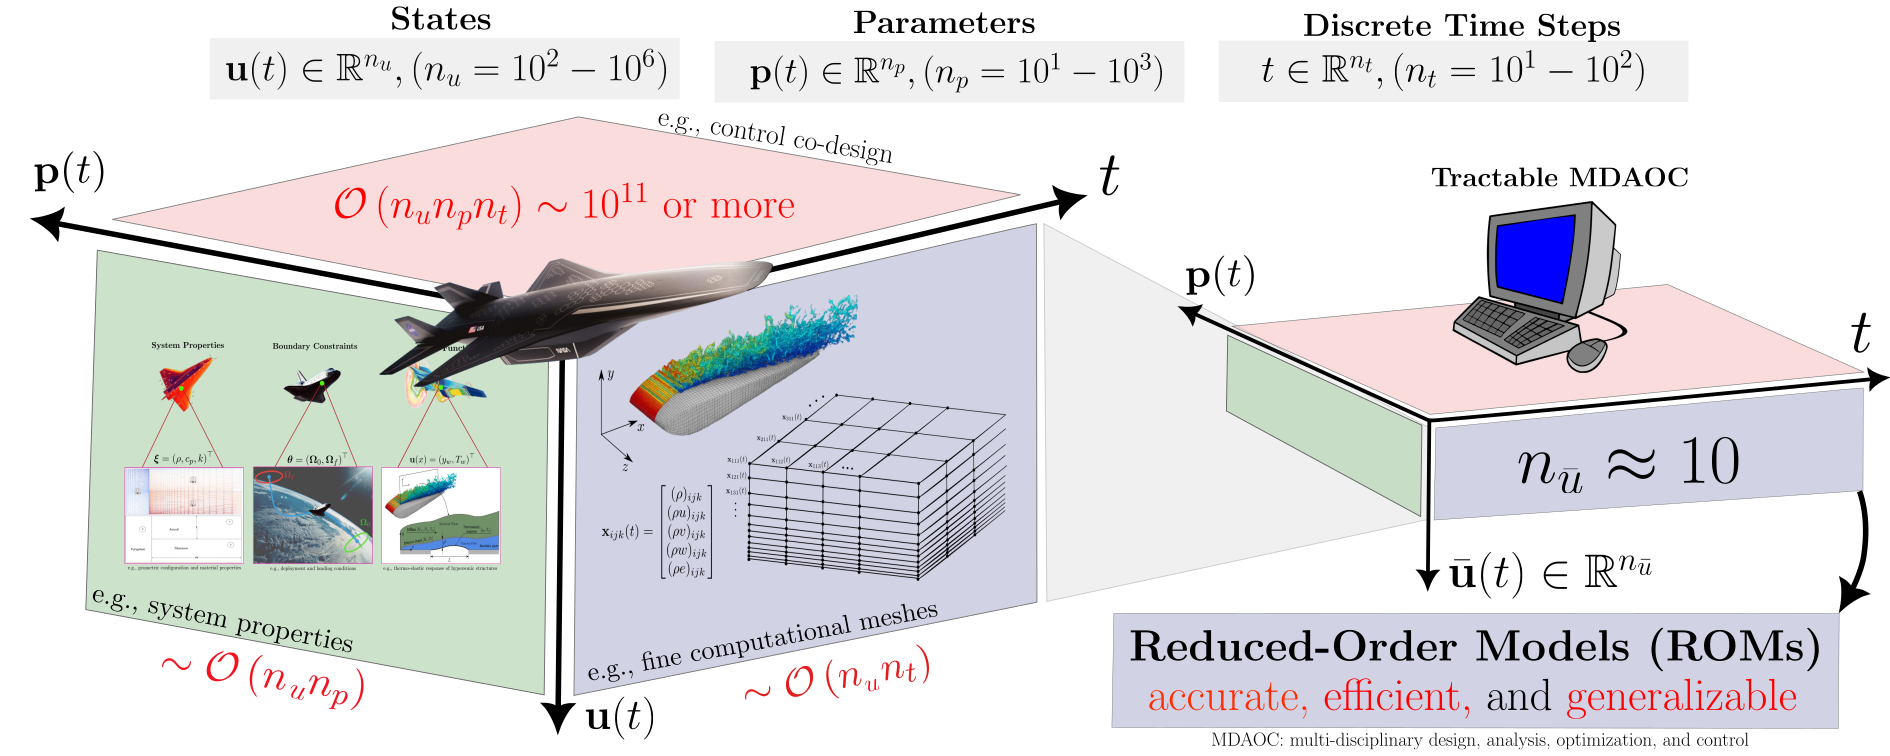
\includegraphics[width=0.95\textwidth]{../figs/introduction/problem_space_10.png}
    \end{figure}
\end{frame}

\begin{frame}{\small How can we balance \textbf{accuracy, efficiency, and generalizability} with little data?}
    \footnotesize
    \begin{columns}
        \begin{column}{0.65\textwidth}
            \begin{figure}
                \centering
                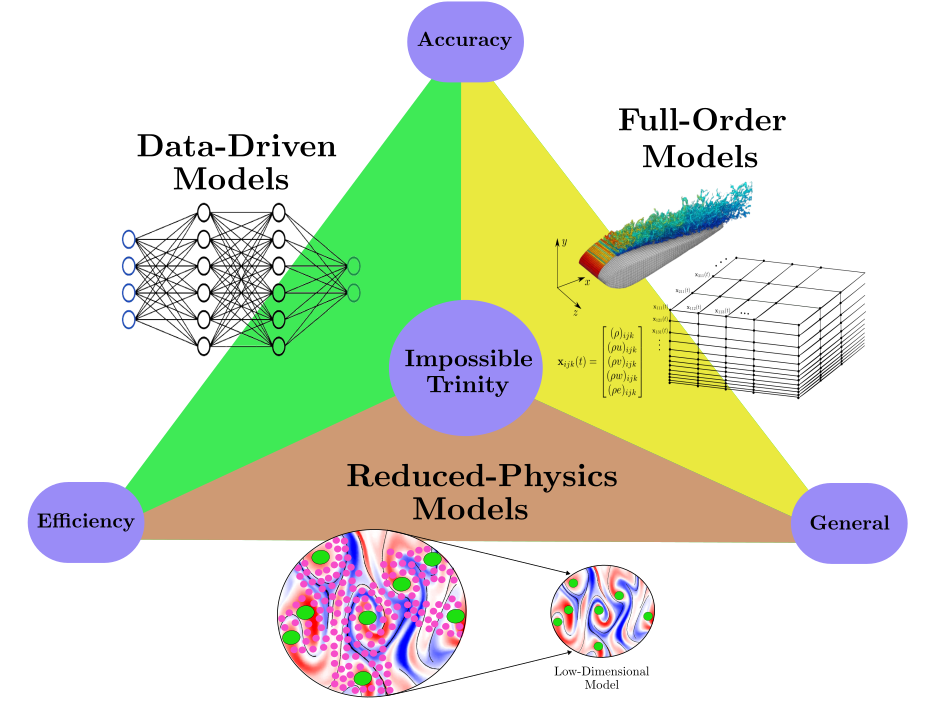
\includegraphics[width=0.8\textwidth]{../figs/introduction/itm_4.png}
            \end{figure}
        \end{column}
        \begin{column}{0.46\textwidth}
            \noindent Remains largely \textbf{unresolved} because,
            \begin{itemize}
                \item \textbf{FEMs}: too many states,
                \item \textbf{RPMs}: overly simplified problems,
                \item \textbf{NNs}: need too much data,
            \end{itemize}
        \end{column}
    \end{columns}
    \begin{center}
        {\tiny ITM: Impossible Trinity of Modeling, FEM: finite-element method, RPM: reduced-physics model, NN: neural network}
    \end{center}
\end{frame}

\begin{frame}{\small How can we balance \textbf{accuracy, efficiency, and generalizability} with little data?}
    \footnotesize
    \begin{columns}
        \begin{column}{0.65\textwidth}
            \begin{figure}
                \centering
                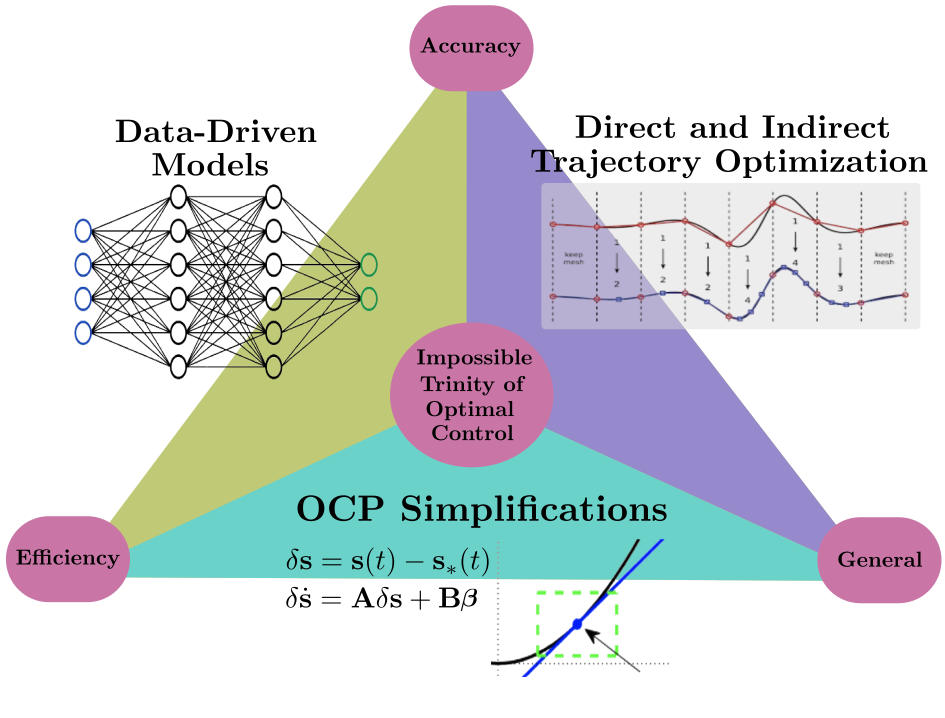
\includegraphics[width=0.8\textwidth]{../figs/introduction/itoc_4.png}
            \end{figure}
        \end{column}
        \hspace*{-0.2in}
        \begin{column}{0.5\textwidth}
            \noindent Remains largely \textbf{unresolved} because,
            \begin{itemize}
                \item \textbf{TO}: need discretization and optimization,
                \item \textbf{NNs}: biased towards training data,
                \item \textbf{Linearizations}: not the original problem
            \end{itemize}
        \end{column}
    \end{columns}
    \begin{center}
        {\tiny ITOC: Impossible Trinity of Optimal Control, TO: trajectory optimization, OCP: optimal control problem}
    \end{center}
\end{frame}


\begin{frame}{\small Objectives of research are \textbf{to solve the ITM and ITOC simultaneously},}
    \footnotesize
    \begin{figure}
        \centering
        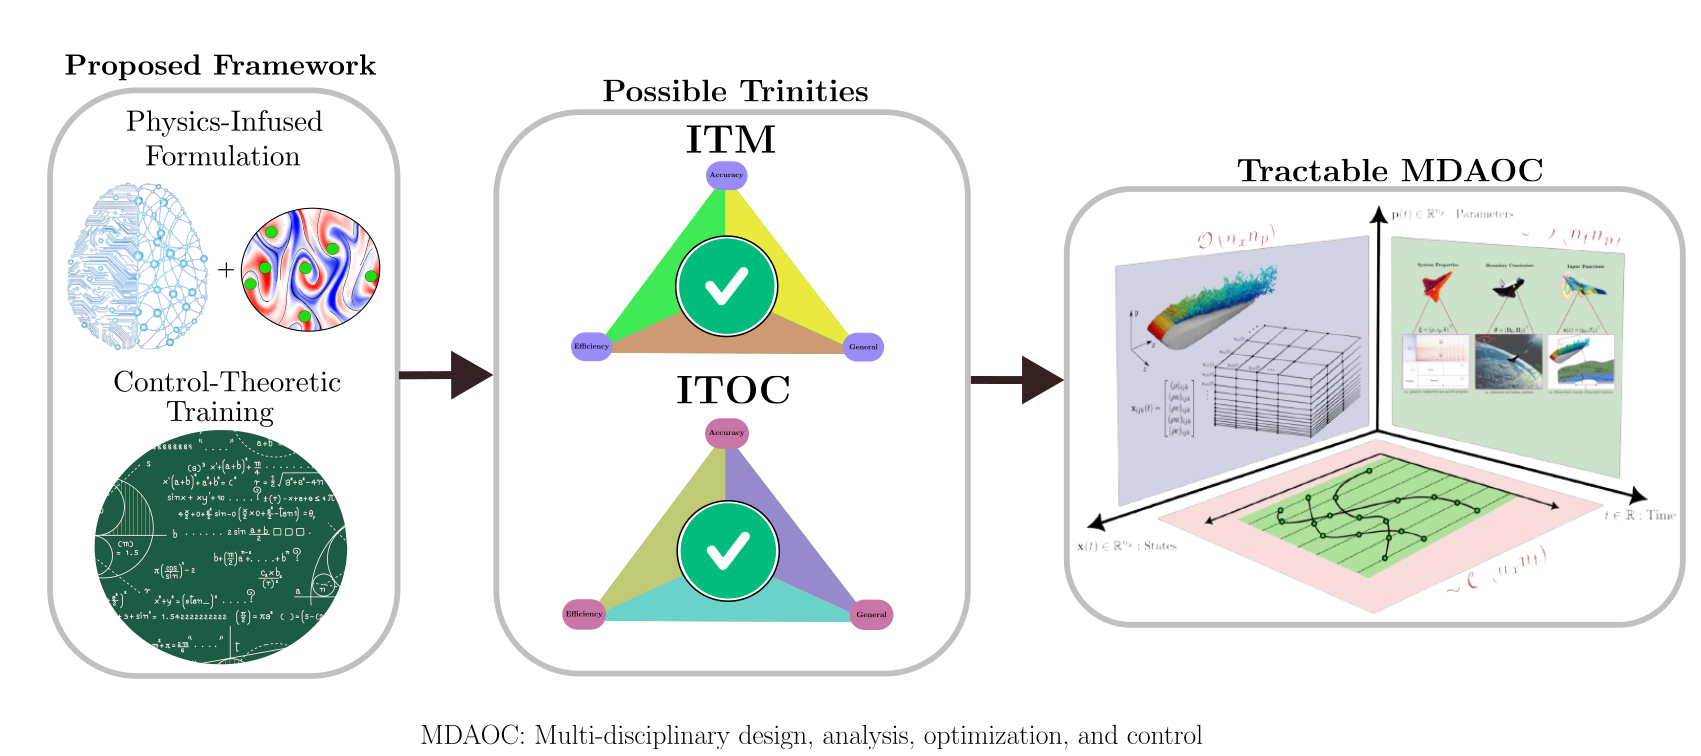
\includegraphics[width=0.95\textwidth]{../figs/introduction/objectives_3.png}
    \end{figure}
\end{frame}

